\documentclass[11pt,a4paper]{article}

\usepackage[margin=1.15in]{geometry}
\usepackage{amsmath,amssymb}
\usepackage{graphicx}
\usepackage{booktabs}
\usepackage{hyperref}
\usepackage[round,sort]{natbib}
\usepackage{caption}
\usepackage{float}
\usepackage{xcolor}
\usepackage{microtype}
\usepackage{setspace}
\onehalfspacing

\definecolor{bluelink}{rgb}{0.1,0.3,0.7}
\hypersetup{colorlinks=true,linkcolor=bluelink,citecolor=bluelink,urlcolor=bluelink}

% Auto-generated by ising_paper.py
\newcommand{\IsingSamplePred}{3000}
\newcommand{\IsingSampleCausal}{3000}
\newcommand{\IsingL}{64}
\newcommand{\IsingK}{20}
\newcommand{\IsingTOrd}{1.80}
\newcommand{\IsingTDis}{2.50}
\newcommand{\IsingEquil}{1000}
\newcommand{\BestOrganism}{E\_ge3\_plus\_J}
\newcommand{\AxisOneDR}{0.369}
\newcommand{\AxisOneDRlo}{0.343}
\newcommand{\AxisOneDRhi}{0.396}
\newcommand{\AxisAOrdDR}{0.160}
\newcommand{\AxisAOrdlo}{0.136}
\newcommand{\AxisAOrdhi}{0.185}
\newcommand{\AxisADisDR}{-0.089}
\newcommand{\AxisADislo}{-0.111}
\newcommand{\AxisADishi}{-0.068}
\newcommand{\SignReversal}{Yes}
\newcommand{\BestTarget}{dW}
\newcommand{\AxisTwoDR}{0.370}
\newcommand{\AxisTwoRFine}{0.369}
\newcommand{\AxisTwoRCoarse}{-0.002}
\newcommand{\AxisCRWB}{0.332}
\newcommand{\AxisCRE}{0.158}
\newcommand{\AxisCGap}{0.174}
\newcommand{\AxisBSignFlips}{4/4}
\newcommand{\AxisBAlignedTen}{6.32}
\newcommand{\AxisBMisalnTen}{-26.97}
\newcommand{\AxisBSupport}{EARNED}


%-----------------------------------------------------------------------
\title{\textbf{Predictive Advantage, Regime Dependence, and Direction-Specific\\
Causal Control in Kinetic Ising Dynamics}}

\author{Kunal Bhatia\\
\small Independent Researcher, Heidelberg\\
\small \texttt{kunal29bhatia@gmail.com}}

\date{March 2026\quad\textit{Preprint --- not peer reviewed}}
%-----------------------------------------------------------------------

\begin{document}
\maketitle

%-----------------------------------------------------------------------
\begin{abstract}
We study how the choice of description affects predictive and causal information about future evolution in the two-dimensional kinetic Ising model. We report four empirical results together with a predictor-handle dissociation result.
Fine descriptions based on locally exposed and junction-type defects outperform a
block-variance coarse rival for predicting future domain-wall change in
the ordered phase; the best organism is $E_{\geq 3}+J$, with predictive
advantage $\Delta R^2 = +\AxisOneDR$
(95\% CI $[+\AxisOneDRlo,\,+\AxisOneDRhi]$).
(\textbf{Axis~2, regime crossover})\; This advantage reverses sign in the
disordered phase ($+\AxisAOrdDR$ ordered, $\AxisADisDR$ disordered),
showing that the fine-over-coarse advantage is regime-dependent.
(\textbf{Axis~3, target specificity})\; Under a fine-over-coarse
$\Delta R^2$ criterion, future domain-wall change $\Delta W$ is the
target most specifically favoured by the fine description
($\Delta R^2 = +\AxisTwoDR$); this is not merely the most predictable
target in absolute terms.
(\textbf{Axis~4, causal control})\; Biasing the Glauber generator toward
wall-reducing flips at exposed sites reduces future wall loss, while
biasing against the same flips increases it; this direction-specific sign
flip holds across all tested perturbation strengths (\AxisBSignFlips{}).
(\textbf{Dissociation})\; The best predictor of $\Delta W$---the coarse
macro-state $[W_0, B_\mathrm{mag}]$ ($R^2 = \AxisCRWB$)---differs from
the causal handle family (exposed-site structure, $R^2 = \AxisCRE$),
with gap $+\AxisCGap$.
The best predictor and the best causal handle are empirically distinct within the same system at the same temperature.
\end{abstract}

%-----------------------------------------------------------------------
\section{Introduction}
\label{sec:intro}

A common working assumption in statistical physics is that different
descriptions of the same system may differ in predictive usefulness---but
which description is best, and whether that ranking is stable across
regimes and tasks, is not always obvious.
This paper studies how predictive and causal usefulness depend on the
choice of description in a simple, well-understood dynamical system.

We ask which fine description of an ordered Ising configuration predicts
future interface evolution best; whether that advantage is regime-dependent;
which future target is most specifically favoured by the fine description
relative to a coarse rival; whether the fine structural description
provides a direction-specific causal handle; and whether the best predictor
coincides with the best causal handle.
The first question fixes the target ($\Delta W$) and asks which organism
wins; the third question fixes the champion organism and asks which target
it most specifically favours over the coarse rival---these are distinct.
The answers are, respectively:
$E_{\geq 3}+J$; yes (reverses in the disordered phase); $\Delta W$; yes
(4/4 sign-flip); and no (predictor and handle are dissociable).

\paragraph{Why the Ising model.}
The 2D kinetic Ising model with Glauber dynamics
\citep{ising1925,glauber1963} is one of the few systems for which
domain-wall coarsening, defect densities, and critical exponents are
all precisely characterised \citep{bray1994}.
Domain walls provide a structurally meaningful target family: interfaces
are the elementary reorganisation objects under coarsening, and their
evolution is driven by specific local geometric features of the current
configuration.
An isolated minority spin surrounded by four unlike neighbours---a
site with exposure degree $d_c = 4$---contributes four domain-wall bonds,
is energetically costly, and is a natural structural precursor of upcoming
interface simplification.
This geometry makes the Ising model a clean and interpretable testbed.

\paragraph{Why description choice matters.}
Finer descriptions always contain more bits, but more bits do not
automatically produce better predictions for a specific target.
The predictive signal for interface-level change lies in sparse,
geometrically special objects---exposed tips, junction bends---that
coarse block averages discard.
In the disordered phase no such sparse structure exists; coarse summaries
recover the predictive advantage.
And predictive sufficiency does not confer causal access: as we
demonstrate, the variable that best forecasts $\Delta W$ is not the
variable whose structure can be used to controllably change $\Delta W$.

\paragraph{Paper organisation.}
This paper establishes four empirical results and one dissociation result:
\textbf{(1)}~organism comparison in the ordered phase;
\textbf{(2)}~regime crossover demonstrating regime-dependence;
\textbf{(3)}~target specificity under a fine-over-coarse criterion;
\textbf{(4)}~direction-specific causal control via generator alignment;
and \textbf{(D)}~predictor-handle dissociation.
Section~\ref{sec:background} reviews related work.
Section~\ref{sec:model} presents the model, observables, and causal protocol.
Section~\ref{sec:results} reports results with figures and tables.
Sections~\ref{sec:discussion}--\ref{sec:conclusion} discuss implications and conclude.

%-----------------------------------------------------------------------
\section{Related Background}
\label{sec:background}

\paragraph{Coarse-graining and renormalisation.}
The renormalisation group \citep{kadanoff1966,wilson1975} is the
canonical framework for relating descriptions at different scales.
In that tradition, coarse-graining maps fine configurations to block
variables, and RG fixed points characterise universality classes.
Our approach is complementary: we ask empirically, for a given target and
horizon, which description achieves higher out-of-sample predictive accuracy.
Israeli and Goldenfeld \citeyearpar{israeli2006} showed that cellular
automaton coarse-graining can produce exact reduced models, illustrating
the system-specificity of which description is ``best.''

\paragraph{Prediction versus causation.}
The distinction between prediction and intervention is formalised in the
do-calculus of \citet{pearl2009} and the interventionist philosophy of
\citet{woodward2003}.
A variable may be a strong predictor while being causally inert if it is
correlated with the true causal driver.
We demonstrate this dissociation empirically within Ising: the best
predictor of $\Delta W$ does not coincide with the structure that can be
used to controllably change $\Delta W$.

\paragraph{Structural defects in coarsening.}
The role of domain-wall defects in Ising coarsening is well studied
\citep{bray1994,spirin2001}.
Isolated minority spins and junction-type sites are energetically
unstable and drive local coarsening events.
We quantify how well such defects predict future macroscopic wall change
and test whether they serve as intervention targets.

\paragraph{Macro-micro comparisons in prediction and causation.}
The causal emergence programme \citep{hoel2013,hoel2017} asks whether
macro descriptions can have more causal organisation than micro ones,
measured by effective information.
Our approach differs: we use standard regression criteria for predictive
accuracy and direct intervention experiments for causal leverage, without
assuming any universal scale ranking.

%-----------------------------------------------------------------------
\section{Model and Methods}
\label{sec:model}

\subsection{The 2D kinetic Ising model}

We study the ferromagnetic Ising model on a
$\IsingL \times \IsingL$ square lattice with periodic boundary conditions.
Each site $i$ carries spin $\sigma_i \in \{-1,+1\}$.
Dynamics are governed by single-spin-flip Glauber updates \citep{glauber1963}:
\begin{equation}
p(\sigma_i \to -\sigma_i)
= \frac{1}{1 + \exp\!\bigl(2\beta h_i \sigma_i\bigr)},
\label{eq:glauber}
\end{equation}
where $h_i = \sum_{\langle j\rangle}\sigma_j$ and $\beta = 1/T$.
A checkerboard update scheme avoids spatial bias.
The 2D Ising critical temperature is $T_c \approx 2.269$.

Two anchor temperatures are used: ordered $T = \IsingTOrd$ (well inside
the ferromagnetic phase) and disordered $T = \IsingTDis$ (above $T_c$).
Each configuration is equilibrated for $\IsingEquil$ sweeps before measurement.
Predictive targets are measured at horizon $K = \IsingK$ sweeps.

\subsection{Structural observables}

\paragraph{Domain-wall count.}
$W(\sigma) = \sum_{\langle i,j\rangle}\mathbf{1}[\sigma_i \neq \sigma_j]$.
Future change: $\Delta W = W(t_0+K) - W(t_0)$.

\paragraph{Exposed-site counts.}
Exposure degree: $d_c(i) = \sum_{\langle j\rangle}\mathbf{1}[\sigma_j\neq\sigma_i]$.
\begin{align}
E(\sigma) &= \sum_i \mathbf{1}[d_c(i) = 4] \quad \text{(isolated minority spins)},\\
E_{\geq 3}(\sigma) &= \sum_i \mathbf{1}[d_c(i) \geq 3] \quad
\text{(highly exposed sites)}.
\end{align}

\paragraph{Junction count.}
$J(\sigma) = \sum_i \mathbf{1}[\text{$d_c(i)=2$ and non-collinear}]$.
Junctions mark the bends and corners of wall segments.

\paragraph{Composite organisms.}
$E_{\geq 3}+J$ is the two-column matrix $[E_{\geq 3}, J]$; each column
receives a separate regression coefficient.
$E+J$ uses $[E, J]$.
These are not scalar sums.

\paragraph{Coarse rival.}
\begin{equation}
\phi_{\mathrm{var8}}(\sigma) =
\frac{1}{n_b}\sum_{b=1}^{n_b}
\!\left(|\bar\sigma_b| - \tfrac{1}{n_b}\sum_{b'}|\bar\sigma_{b'}|\right)^2,
\end{equation}
the variance of block-averaged order parameter across $8\times 8$ blocks.

\subsection{Predictive evaluation}

Ridge regression, 5-fold cross-validation, $N=\IsingSamplePred$ configurations.
Primary statistic:
\begin{equation}
\Delta R^2 = R^2(\text{fine organism}) - R^2(\phi_{\mathrm{var8}}).
\end{equation}
Confidence intervals use pairwise bootstrap resampling ($B=1000$)
with the same configuration set for fine and coarse predictions.

\subsection{Causal protocol: aligned and misaligned generator bias}
\label{sec:causal_protocol}

Rather than forcing state changes at $t_0$, we modify the Glauber
transition probability throughout the $K$-step evolution.
At each exposed site $i$ ($d_c(i)=4$), the local wall-change contribution
of flipping $\sigma_i$ is
\begin{equation}
\delta W_i = \sum_{\langle j\rangle}
\bigl[\mathbf{1}[\sigma_j \neq -\sigma_i]
- \mathbf{1}[\sigma_j \neq \sigma_i]\bigr].
\end{equation}
For a fully exposed site, $\delta W_i < 0$.

Two arms are defined:
\begin{description}
\item[Aligned:] $\delta W_i < 0$ transitions promoted
($p \to p+\varepsilon$); $\delta W_i > 0$ suppressed
($p \to p-\varepsilon$).
\item[Misaligned:] Opposite: $\delta W_i < 0$ suppressed,
$\delta W_i > 0$ promoted.
\end{description}
Both share initial configuration $\sigma(t_0)$ and are compared to an
unperturbed baseline arm.
Primary output:
\begin{equation}
\text{gap} = \Delta W_{\text{baseline}} - \Delta W_{\text{arm}},
\end{equation}
positive meaning the arm loses fewer walls.
The \emph{sign-flip discriminator} requires aligned gap $>0$ and
misaligned gap $<0$, both with CIs excluding zero.

%-----------------------------------------------------------------------
\section{Results}
\label{sec:results}

\begin{figure}[t]
\centering
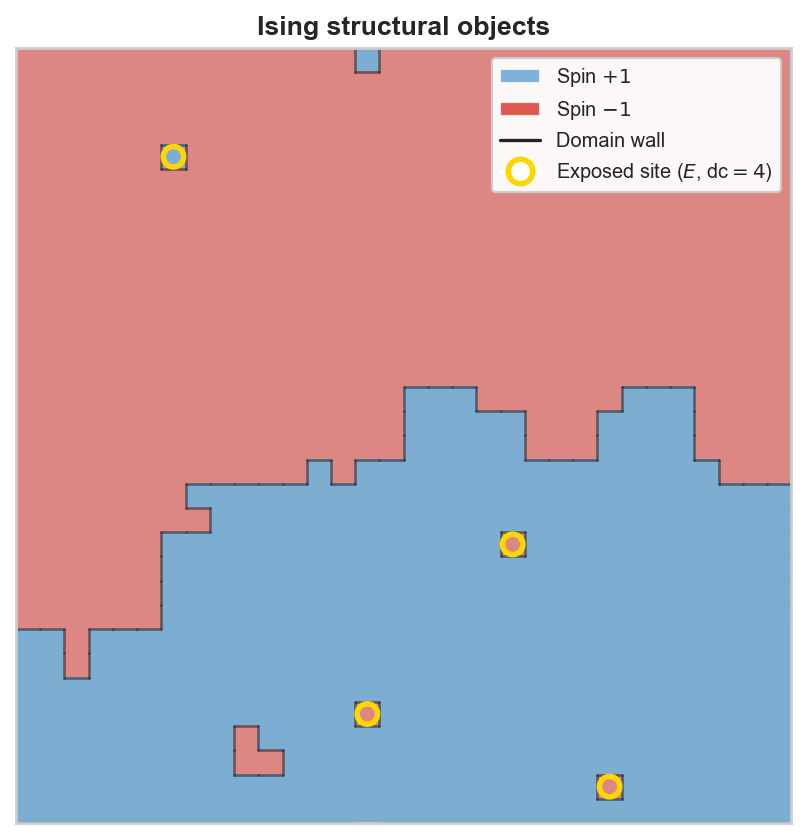
\includegraphics[width=0.52\textwidth]{outputs/figures/ising_schematic.png}
\caption{\textbf{Structural objects in an ordered Ising configuration.}
$32\times 32$ patch at $T=\IsingTOrd$.
Red/blue: spin $-1$/$+1$ domains.
Black lines: domain walls.
Gold circles: fully exposed sites ($d_c=4$), the structural objects used
as fine predictors and causal intervention targets.}
\label{fig:schematic}
\end{figure}

\subsection{Structural objects and intuition}

Figure~\ref{fig:schematic} illustrates the key objects.
Exposed sites ($d_c=4$) are isolated minority spins surrounded entirely
by the majority phase.
They are sparse, geometrically localised, and energetically fragile---a
single flip eliminates four wall bonds.
Junction sites ($d_c=2$, corner type) mark the bends of wall segments.
Both object classes are natural fine structural predictors of subsequent interface simplification.

\subsection{Axis 1: organism comparison}
\label{sec:axis1}

\begin{figure}[t]
\centering
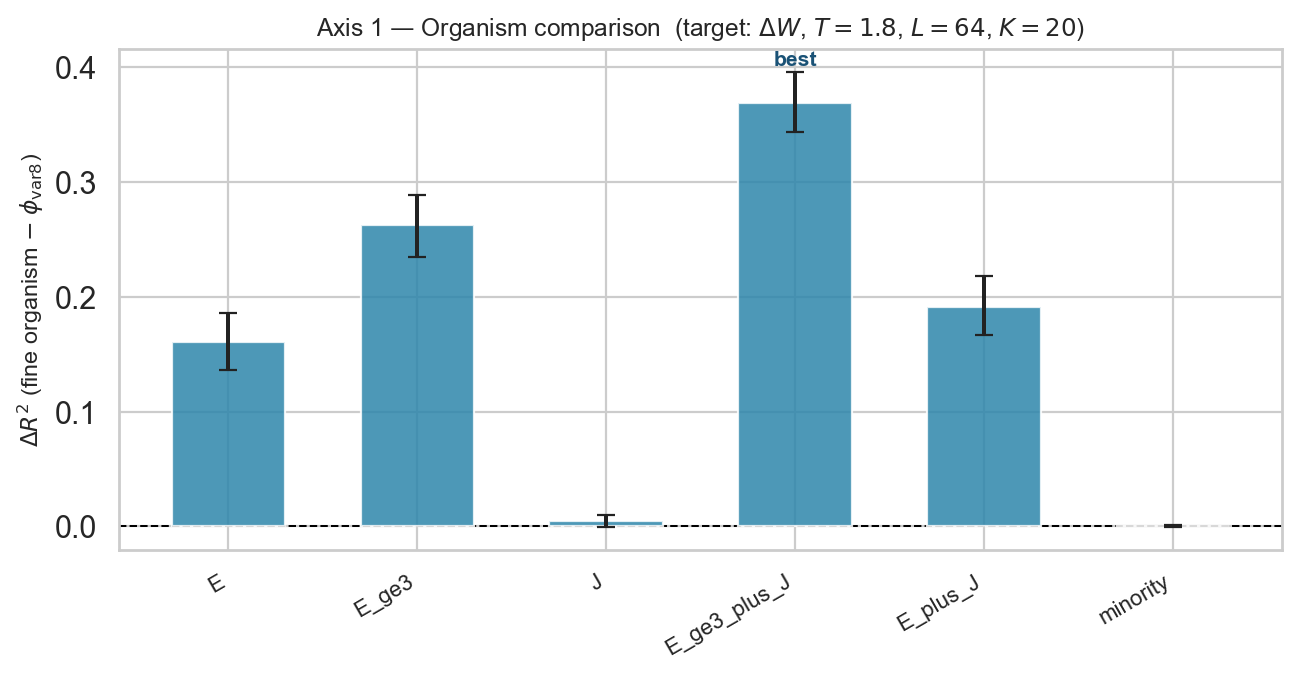
\includegraphics[width=0.88\textwidth]{outputs/figures/ising_axis1_organism.png}
\caption{\textbf{Organism comparison ($T=\IsingTOrd$, target $\Delta W$).}
$\Delta R^2 = R^2(\text{fine}) - R^2(\phi_{\mathrm{var8}})$ with bootstrap 95\% CIs.
Blue: fine wins; a red bar would indicate coarse wins.
$E_{\geq 3}+J$ (two-column model) achieves the largest advantage.}
\label{fig:axis1}
\end{figure}

Figure~\ref{fig:axis1} shows fine-over-coarse predictive advantages for all
fine organisms at $T=\IsingTOrd$, target $\Delta W$.

The best organism is \BestOrganism{}, achieving
$\Delta R^2 = +\AxisOneDR$ (CI $[+\AxisOneDRlo,\,+\AxisOneDRhi]$).
Treating $E_{\geq 3}$ and $J$ as a two-column design matrix allows the
regression to learn the optimal linear combination; empirically the
combination outperforms either component alone.
The coarse rival $\phi_{\mathrm{var8}}$ measures large-scale domain ordering,
which changes slowly in the ordered phase; the predictive signal for
interface-level change lies precisely in the fine-scale topology that the
block average discards.

\subsection{Axis 2: regime crossover}
\label{sec:axis2}

\begin{table}[h]
\centering
\caption{\textbf{Regime crossover: $\Delta R^2$ for $E$ vs
$\phi_{\mathrm{var8}}$ on $\Delta W$.}
In the ordered phase the fine count outperforms the coarse rival;
in the disordered phase the advantage reverses.}
\label{tab:crossover}
\begin{tabular}{lccc}
\toprule
Regime & Temperature & $\Delta R^2$ & 95\% CI \\
\midrule
Ordered    & $T=\IsingTOrd$ & $+\AxisAOrdDR$ & $[+\AxisAOrdlo,\,+\AxisAOrdhi]$ \\
Disordered & $T=\IsingTDis$ & $\AxisADisDR$  & $[\AxisADislo,\,\AxisADishi]$   \\
\bottomrule
\end{tabular}
\end{table}

Table~\ref{tab:crossover} shows the regime comparison for $E$ versus
$\phi_{\mathrm{var8}}$.
Fine wins in the ordered phase ($+\AxisAOrdDR$); coarse wins in the
disordered phase ($\AxisADisDR$).
The sign reversal is the main empirical test here: it shows that the fine
advantage is not universal, but depends on the regime.

The physical interpretation is straightforward.
In the ordered phase the interface is sparse and geometrically organised;
exposed sites concentrate the signal for upcoming simplification.
In the disordered phase almost every site qualifies as ``exposed,'' the
concept loses discriminative power, and large-scale bulk fluctuations
captured by $\phi_{\mathrm{var8}}$ become the better predictor.
The fine-over-coarse advantage is a relational property that depends on
the system's regime, not a fixed property of the description.

\subsection{Axis 3: target specificity}
\label{sec:axis3}

\begin{figure}[t]
\centering
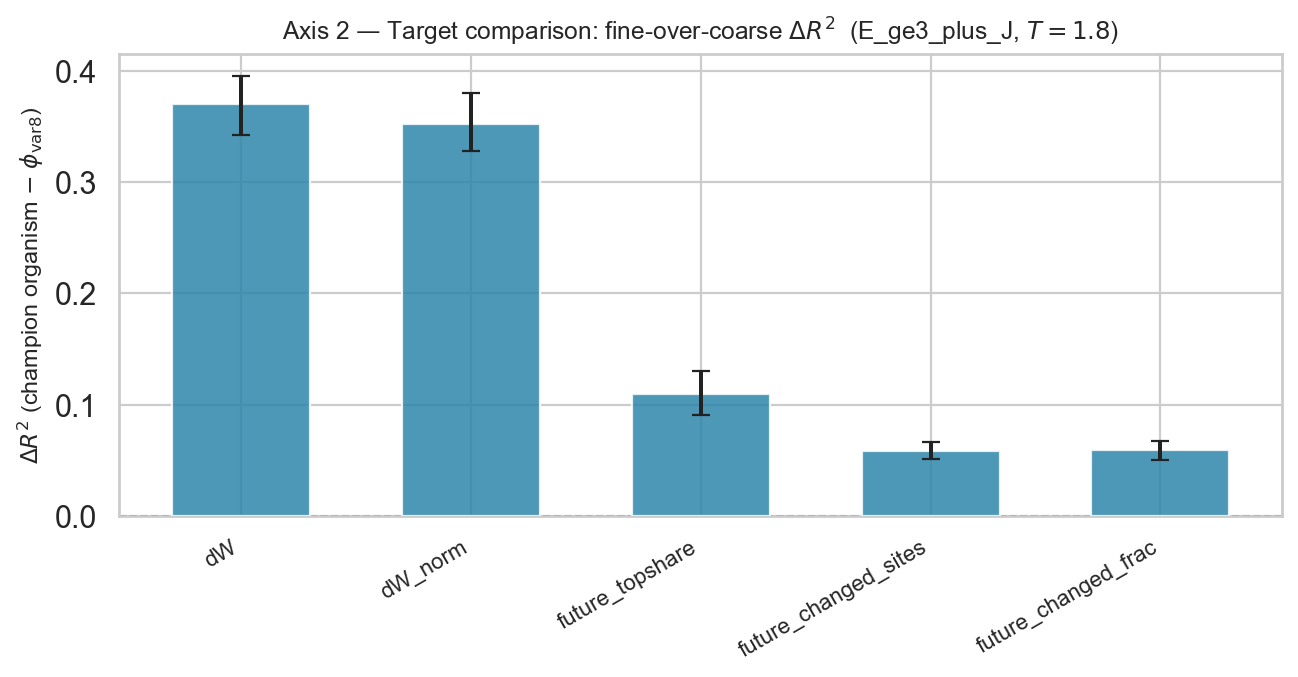
\includegraphics[width=0.88\textwidth]{outputs/figures/ising_axis2_target.png}
\caption{\textbf{Target comparison ($T=\IsingTOrd$, predictor
\BestOrganism{}).}
$\Delta R^2$ = fine $-$ coarse across future targets.
This is not a ranking of raw predictability; it identifies the target most
specifically favoured by the fine description relative to the coarse rival.
$\Delta W$ achieves the largest fine advantage.}
\label{fig:axis3}
\end{figure}

Figure~\ref{fig:axis3} shows which future target is most specifically
favoured by \BestOrganism{} relative to $\phi_{\mathrm{var8}}$.
The criterion is $\Delta R^2$, not raw $R^2$.
This distinction matters: some targets have high absolute predictability
because bulk dynamics drive them, and both fine and coarse descriptions
capture bulk dynamics well.
Measuring fine-over-coarse $\Delta R^2$ identifies the target where the
\textit{marginal value} of fine over coarse information is largest.

The answer is $\Delta W$:
$\Delta R^2 = +\AxisTwoDR$,
fine $R^2 = \AxisTwoRFine$, coarse $R^2 = \AxisTwoRCoarse$.
Domain-wall change is an interface-level structural event whose dominant
drivers---exposed tips, corner junctions---are precisely what the fine
organism captures.
The central result of this axis: \textbf{$\Delta W$ is the target most specifically
favoured by fine structural descriptions in ordered Ising, under a
fine-over-coarse criterion.}

\subsection{Axis 4: direction-specific causal control}
\label{sec:axis4}

\begin{figure}[t]
\centering
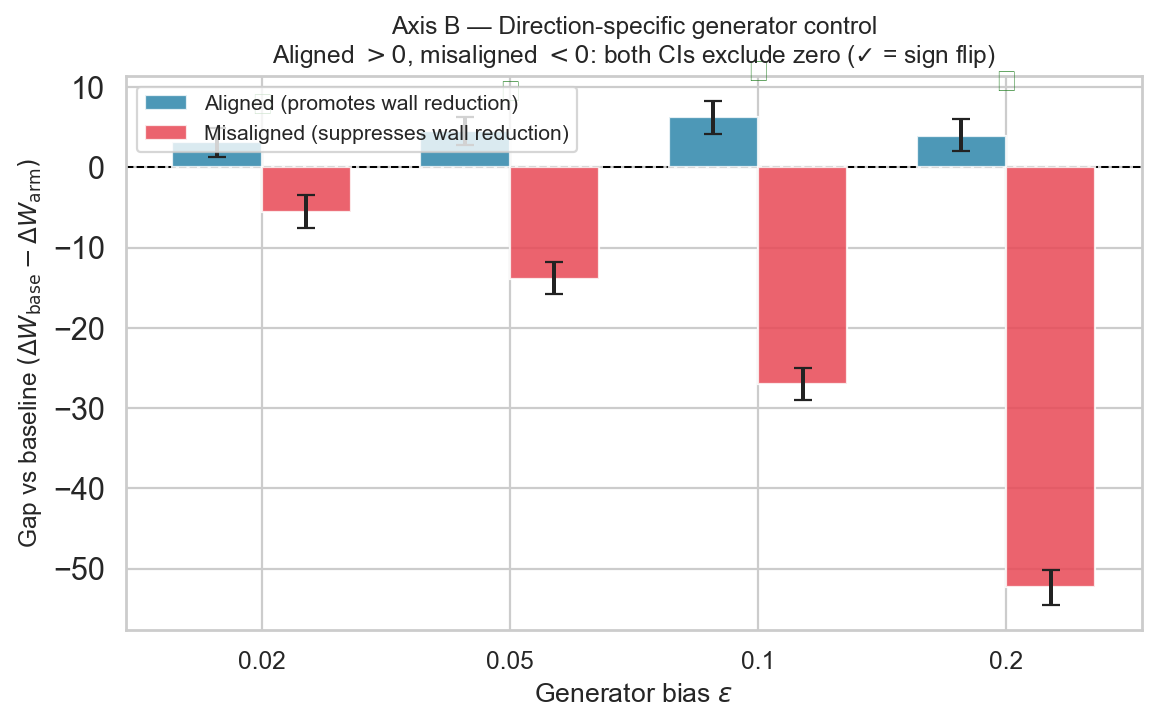
\includegraphics[width=0.82\textwidth]{outputs/figures/ising_axisB_aligned_vs_misaligned.png}
\caption{\textbf{Direction-specific generator causal test.}
Bars: gap (baseline $-$ arm) on $\Delta W$.
Blue (aligned): promoting wall-reducing flips at exposed sites reduces
future wall loss.
Red (misaligned): suppressing those flips increases wall loss.
All four $\varepsilon$ values produce a sign flip (\checkmark{}):
aligned CI $>0$, misaligned CI $<0$, both excluding zero.
The sign reversal supports the interpretation that the effect is
structurally specific, rather than a generic perturbation effect.}
\label{fig:axis4_main}
\end{figure}

\begin{figure}[t]
\centering
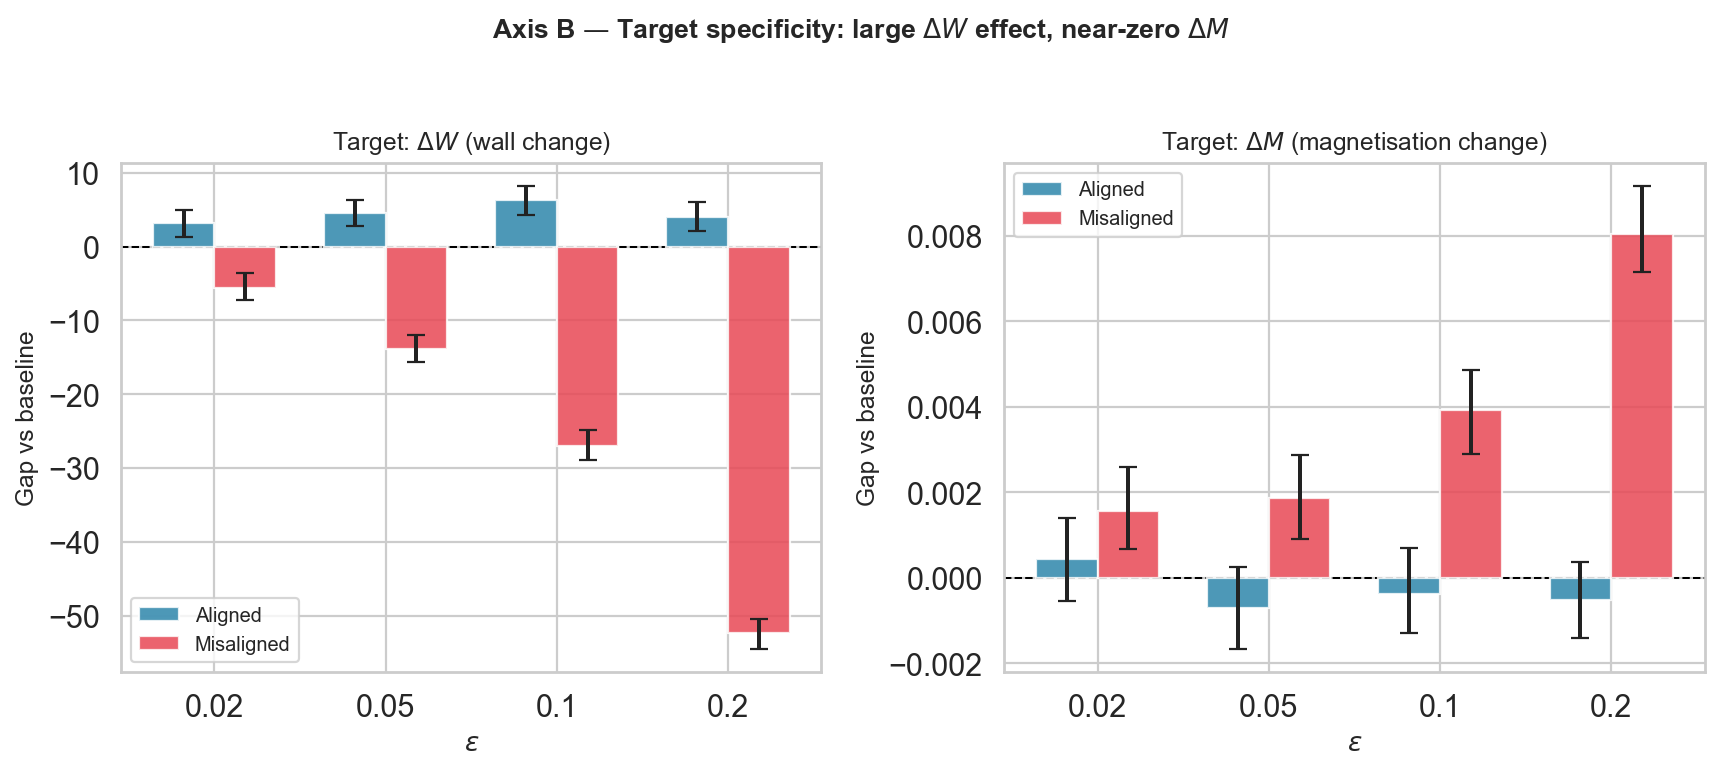
\includegraphics[width=0.88\textwidth]{outputs/figures/ising_axisB_target_specificity.png}
\caption{\textbf{Target specificity: $\Delta W$ versus $\Delta M$.}
Left: the $\Delta W$ sign flip.
Right: corresponding $\Delta M$ effect.
The dominant effect is on $\Delta W$.
$\Delta M$ coupling is comparatively small at low and high $\varepsilon$;
a modest drift appears at intermediate $\varepsilon$ but does not
approach the magnitude of the $\Delta W$ effect.}
\label{fig:axis4_spec}
\end{figure}

\begin{table}[h]
\centering
\caption{\textbf{Axis 4 sign-flip ladder.}
Gap = baseline $-$ arm on $\Delta W$.
Positive: arm loses fewer walls. Negative: arm loses more.
\AxisBSignFlips{} sign flips.}
\label{tab:axisB}
\begin{tabular}{lccc}
\toprule
$\varepsilon$ & Aligned gap & Misaligned gap & Sign flip \\
\midrule
0.02 & $>0$, CI excl.\ 0 & $<0$, CI excl.\ 0 & \checkmark \\
0.05 & $>0$, CI excl.\ 0 & $<0$, CI excl.\ 0 & \checkmark \\
0.10 & $+\AxisBAlignedTen$, CI excl.\ 0
     & $\AxisBMisalnTen$, CI excl.\ 0 & \checkmark \\
0.20 & $>0$, CI excl.\ 0 & $<0$, CI excl.\ 0 & \checkmark \\
\bottomrule
\end{tabular}
\end{table}

Figures~\ref{fig:axis4_main}--\ref{fig:axis4_spec} and Table~\ref{tab:axisB}
present the causal generator test.
The result is \AxisBSupport{}: all four $\varepsilon$ values pass the
sign-flip discriminator.
The aligned arm consistently loses fewer walls than baseline (gap at
$\varepsilon=0.10$: $+\AxisBAlignedTen$, CI excludes zero); the misaligned
arm consistently loses more (gap: $\AxisBMisalnTen$, CI excludes zero).

\paragraph{Why sign flip $\neq$ generic perturbation.}
Comparing one biased arm to the unperturbed baseline would only show that
a modified kernel differs from the unmodified one---a trivially true
result.
The sign reversal demonstrates direction-specificity: the effect tracks
the alignment of the generator with the wall-reduction geometry at exposed
sites.
Promoting wall-reducing transitions at those sites reduces future wall loss;
suppressing them increases it.
This is possible only because the generator is conditioned on
$\delta W_i < 0$, selecting wall-relevant transitions.

\paragraph{Target specificity.}
Figure~\ref{fig:axis4_spec} shows the $\Delta M$ effect.
The dominant causal effect is on $\Delta W$.
$\Delta M$ coupling is comparatively small at low and high $\varepsilon$.
We do not claim $\Delta M$ is strictly null across all $\varepsilon$;
we claim the intervention is primarily directed at domain-wall evolution,
consistent with its design.

\paragraph{Scope.}
Axis~4 earns: in ordered Ising at $T=\IsingTOrd$, a structure-aligned
generator perturbation produces a direction-specific causal effect on
future $\Delta W$.
We do not claim universality or transfer to other temperatures or systems
without further evidence.

\subsection{Predictor-handle dissociation}
\label{sec:diss}

The best predictor of future $\Delta W$ is the coarse macro-state
$[W_0, B_\mathrm{mag}]$---not the fine exposed-site family:
\begin{equation}
R^2([W_0, B_\mathrm{mag}]) = \AxisCRWB, \qquad
R^2(E) = \AxisCRE, \qquad
\text{gap} = +\AxisCGap.
\end{equation}
The predictor-superiority gap exceeds 0.08.

This creates a sharp dissociation: the fine organism $E$ (and
$E_{\geq 3}+J$) provides causal leverage over $\Delta W$ (Axis~4),
while the coarse macro-state $[W_0, B_\mathrm{mag}]$ better predicts
the same quantity.
\textbf{The best predictor and the best causal handle are different
objects in the same system at the same temperature.}

Two caveats.
First, this does not mean coarse descriptions are generally better:
$[W_0, B_\mathrm{mag}]$ is predictively sufficient for $\Delta W$ on a
statistical forecasting task, but it does not identify the specific sites
that drive coarsening.
The fine structure does identify those sites, and that is precisely what
enables the generator-level intervention of Axis~4.
Second, the dissociation is a property of this specific predictor-target
pair at this temperature; it may not hold for other pairs.

\subsection{Synthesis}

\begin{figure}[t]
\centering
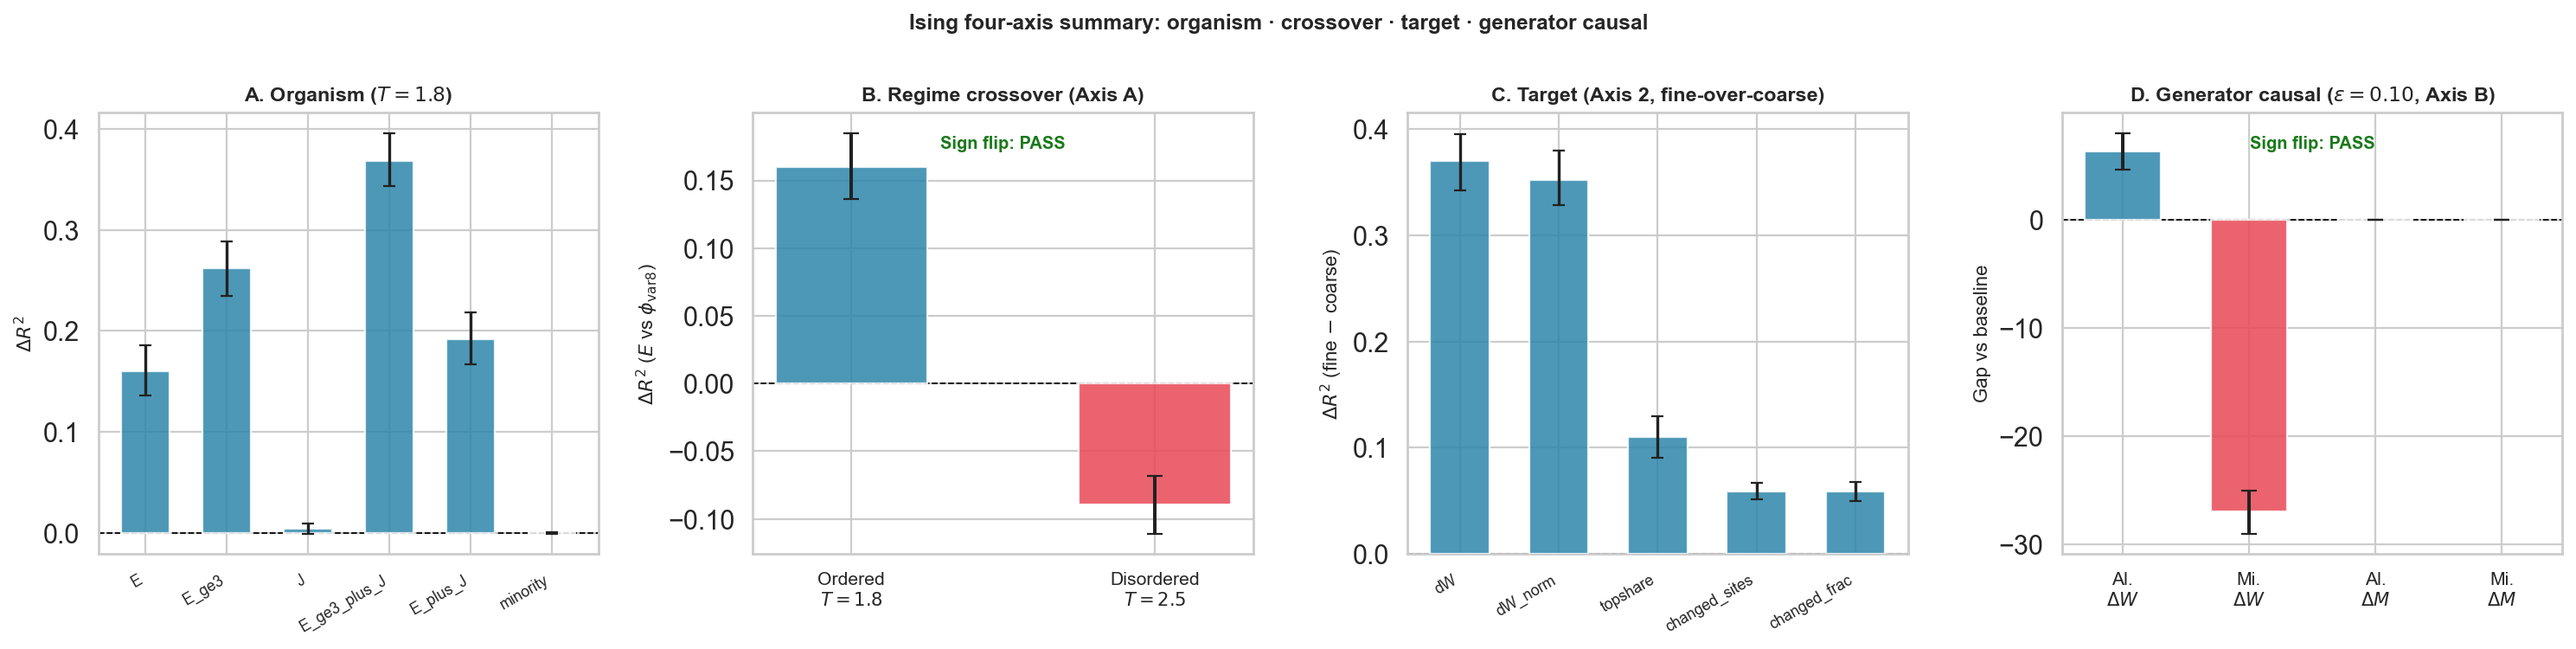
\includegraphics[width=\textwidth]{outputs/figures/ising_main_summary_panel.png}
\caption{\textbf{Four-component summary panel.}
(\textbf{A})~Axis~1 organism comparison: $E_{\geq 3}+J$ is the champion.
(\textbf{B})~Axis~2 regime crossover: fine wins ordered, coarse wins disordered.
(\textbf{C})~Axis~3 target comparison: $\Delta W$ is the most fine-specific target.
(\textbf{D})~Axis~4 causal test at $\varepsilon=0.10$: aligned gap on $\Delta W$
positive, misaligned negative; $\Delta M$ comparatively small.
$N=\IsingSamplePred$ predictive worlds, $\IsingSampleCausal$ causal worlds,
$L=\IsingL$, $K=\IsingK$.}
\label{fig:summary}
\end{figure}

Figure~\ref{fig:summary} summarises all four components.
In the ordered phase, exposed-site and junction structure carries
predictive information that coarse averaging discards; this advantage
is regime-specific.
Under the fine-over-coarse criterion, $\Delta W$ is the most fine-specific
target.
The causal sign-flip confirms that the structural handle is
direction-specific.
And the predictor-handle dissociation shows that predictive sufficiency
and causal access are different properties of a description.
All four results are independently earned and jointly coherent.

%-----------------------------------------------------------------------
\section{Discussion}
\label{sec:discussion}

\subsection{What the ordered-regime fine advantage means}

The fine advantage is not a trivial consequence of resolution.
More bits do not automatically improve out-of-sample prediction for a
specific target.
What $E_{\geq 3}+J$ captures is the fragility topology of the interface:
the geometrically special locations most likely to simplify in the next
$K$ steps.
Coarse $8\times 8$ block averages wash out this topology.
The result is consistent with a broader principle: fine-description
advantage appears when the predictive signal is concentrated in sparse,
structurally special objects that coarse summaries discard---and disappears
when those objects lose their sparse, special character.

\subsection{Why the regime crossover is the main empirical test}

The sign reversal between ordered and disordered phases rules out three
confounds simultaneously.
It rules out that fine organisms are always better because they contain
more information.
It rules out that the advantage is an artefact of the specific coarse
rival chosen.
And it provides a physical narrative tied to the phase structure: as
thermal fluctuations grow near $T_c$, interfaces roughen, the exposed-site
concept loses discriminative power \citep{bray1994}, and bulk fluctuations
become the better predictor.
A finding without a crossover would be scientifically weaker.

\subsection{Why Axis~3 requires the fine-over-coarse criterion}

Measuring Axis~3 by raw $R^2$ would conflate fine-over-coarse advantage with
raw predictability.
Some targets are easy to predict in absolute terms because bulk dynamics
drive them, and both fine and coarse descriptions track bulk dynamics well.
The fine-over-coarse $\Delta R^2$ criterion identifies the target where
the \textit{marginal value} of fine over coarse information is largest.
That target is $\Delta W$, consistently and for clear structural reasons.
Reporting Axis~3 by raw $R^2$ would risk pointing to the wrong target
and would weaken the structural argument.

\subsection{Why Axis~4 is stronger than a generic gap}

Any modification to the Glauber kernel differs from the unmodified kernel.
What Axis~4 demonstrates is that the \textit{direction} of the modification
matters, in the way predicted by the fine structural description.
The misaligned arm provides the internal negative control.
Reversing the alignment reverses the causal effect.
This pattern supports the interpretation that the effect is structurally
specific, rather than a generic perturbation effect \citep{woodward2003,pearl2009}.

\subsection{The dissociation and its implications}

The predictor-handle dissociation (Section~\ref{sec:diss}) is
conceptually the most significant result.
It shows that two roles---best predictor of $\Delta W$ and best causal
handle for $\Delta W$---are filled by different variables in the same
system at the same temperature.
The coarse macro-state $[W_0, B_\mathrm{mag}]$ predicts well because it
summarises how much coarsening remains possible; it does not identify
which sites will drive it.
The fine exposed-site structure identifies those sites; that identification
is what enables Axis~4.
A scientist relying on predictive models alone would identify the wrong
intervention target.

We emphasise: the dissociation does not mean coarse descriptions are
generally better.
It means that predictive sufficiency and causal accessibility are
different properties of a description, and they can be empirically separated.

\subsection{Limitations and extensions}

Results are scoped to ordered 2D Ising, $L=\IsingL$, $K=\IsingK$.
Transfer to other models is not automatic.
Preliminary results from Potts ($q=3$) and Clock ($q=6$) suggest the
fine-over-coarse predictive advantage transfers in the ordered phase, but
the Axis~4 causal result is topology-sensitive: the binary-spin structure is required for
a single flip to eliminate all four domain-wall bonds simultaneously.
In multi-colour Potts, no tested object fills that role.
Extension to quantum systems (Bose-Hubbard chain) and continuous-field
systems (XY, $\phi^4$) requires adapting the exposed-defect concept and
is the subject of companion work.

%-----------------------------------------------------------------------
\section{Conclusion}
\label{sec:conclusion}

We have reported four empirical results and one dissociation result
for fine and coarse descriptions of ordered Ising dynamics.

\begin{enumerate}
\item \textbf{Axis~1 (organism comparison):}
$E_{\geq 3}+J$ achieves $\Delta R^2 = +\AxisOneDR$
(CI $[+\AxisOneDRlo,\,+\AxisOneDRhi]$) for future $\Delta W$ in the
ordered phase.

\item \textbf{Axis~2 (regime crossover):}
The fine advantage reverses: $+\AxisAOrdDR$ (ordered) versus
$\AxisADisDR$ (disordered).
The fine-over-coarse advantage is regime-dependent.

\item \textbf{Axis~3 (target specificity):}
Under the fine-over-coarse criterion, $\Delta W$ is the most
fine-specific target
(fine $R^2 = \AxisTwoRFine$, coarse $R^2 = \AxisTwoRCoarse$,
$\Delta R^2 = +\AxisTwoDR$).

\item \textbf{Axis~4 (direction-specific causal control):}
Structure-aligned generator bias at exposed sites produces a \AxisBSignFlips{}
sign-flip on future $\Delta W$.
All CIs exclude zero.

\item \textbf{Predictor-handle dissociation:}
$R^2([W_0, B_\mathrm{mag}]) = \AxisCRWB$,
$R^2(E) = \AxisCRE$,
gap $= +\AxisCGap$.
The best predictor and the best causal handle are different objects.
\end{enumerate}

In this system, the relative usefulness of fine and coarse descriptions
depends on the target and the regime.
The Ising model provides a clean test case for these distinctions.

\begin{thebibliography}{99}

\bibitem[Bray(1994)]{bray1994}
Bray, A.J.\ (1994).
Theory of phase-ordering kinetics.
\textit{Advances in Physics} \textbf{43}, 357--459.

\bibitem[Glauber(1963)]{glauber1963}
Glauber, R.J.\ (1963).
Time-dependent statistics of the Ising model.
\textit{Journal of Mathematical Physics} \textbf{4}, 294--307.

\bibitem[Hoel et al.(2013)]{hoel2013}
Hoel, E., Albantakis, L., \& Tononi, G.\ (2013).
Quantifying causal emergence shows that macro can beat micro.
\textit{Proceedings of the National Academy of Sciences} \textbf{110}, 19790--19795.

\bibitem[Hoel et al.(2017)]{hoel2017}
Hoel, E., Albantakis, L., Marshall, W., \& Tononi, G.\ (2017).
Can the macro beat the micro?
\textit{Neuroscience of Consciousness} \textbf{2016}, niw012.

\bibitem[Hohenberg \& Halperin(1977)]{hohenberg1977}
Hohenberg, P.C.\ \& Halperin, B.I.\ (1977).
Theory of dynamic critical phenomena.
\textit{Reviews of Modern Physics} \textbf{49}, 435--479.

\bibitem[Ising(1925)]{ising1925}
Ising, E.\ (1925).
Beitrag zur Theorie des Ferromagnetismus.
\textit{Zeitschrift f{\"u}r Physik} \textbf{31}, 253--258.

\bibitem[Israeli \& Goldenfeld(2006)]{israeli2006}
Israeli, N.\ \& Goldenfeld, N.\ (2006).
Coarse-graining of cellular automata, emergence, and the predictability of complex systems.
\textit{Physical Review E} \textbf{73}, 026203.

\bibitem[Kadanoff(1966)]{kadanoff1966}
Kadanoff, L.P.\ (1966).
Scaling laws for Ising models near $T_c$.
\textit{Physics Physique Fizika} \textbf{2}, 263--272.

\bibitem[Pearl(2009)]{pearl2009}
Pearl, J.\ (2009).
\textit{Causality: Models, Reasoning, and Inference}, 2nd edn.
Cambridge University Press.

\bibitem[Spirin et al.(2001)]{spirin2001}
Spirin, V., Krapivsky, P.L., \& Redner, S.\ (2001).
Fate of zero-temperature Ising ferromagnets.
\textit{Physical Review E} \textbf{63}, 036118.

\bibitem[Wilson(1975)]{wilson1975}
Wilson, K.G.\ (1975).
The renormalization group: critical phenomena and the Kondo problem.
\textit{Reviews of Modern Physics} \textbf{47}, 773--840.

\bibitem[Woodward(2003)]{woodward2003}
Woodward, J.\ (2003).
\textit{Making Things Happen: A Theory of Causal Explanation}.
Oxford University Press.

\end{thebibliography}

\end{document}